%%%%%%%%%%%%%%%%%%%%%%%%%%%%%%%%%%%%%%%%%%%%%%%%%%%%%%%%%%%%%%%%%%%%%%%%%%%%%%%%%
% Plantilla para el Avance del curso FS0751/FS0624		%					
% RECOMENDACIÓN: hagan una copia de la plantilla para sus trabajos.																%
%%%%%%%%%%%%%%%%%%%%%%%%%%%%%%%%%%%%%%%%%%%%%%%%%%%%%%%%%%%%%%%%%%%%%%%%%%%%%%%%%		
% PREÁMBULO												%
% El preámbulo en un documento LaTeX es el conjunto de comandos que preceden 			%
% la línea \begin{document} line. Contiene la línea \documentclass para cargar			%
% las definiciones REVTeK-4 y varias otras líneas \usepackage para cargar				%
% otros paquetes.																		%
%																						%
% ADVERTENCIA A LOS ESTUDIANTES: El preámbulo contiene un conjunto de paquetes necesarios para un compilado apropiado. Se recomienda no eliminar paquetes por completo aunque piense que no los necesita, coméntelos. Ud puede también agregar paquetes según lo vea conveniente.
%%%%%%%%%%%%%%%%%%%%%%%%%%%%%%%%%%%%%%%%%%%%%%%%%%%%%%%%%%%%%%%%%%%%%%%%%%%%%%%%%

\documentclass[aps,twocolumn,secnumarabic,nobalancelastpage,amsmath,amssymb,
nofootinbib]{revtex4}

% nofootinbib es otra clase de documento que permite colocar notas al pie de
% página en la página donde ocurre, en lugar de al final del artículo. De esta
% manera es más fácil de leer!

% secnumarabic es una manera particular de identificar la secciones por número.
% para ayudar a la revisión electrónica.

% amsmath and amssymb son necesarias para el ambiente de las subecuaciones, 
% entre otras

\usepackage{graphics}      % especificaciones gráficas estándar
\usepackage{graphicx}      % especificaciones alternativas para lso gráficos
\usepackage{longtable}     % ayuda con las opciones de tablas grandes
\usepackage{url}           % para referencias en línea
\usepackage{bm}            % paquete especial 'bold-math'
\usepackage[utf8]{inputenc}
\usepackage[spanish, es-tabla]{babel}% para que utilice las reglas gramaticales del español
						   % y reconozca las tildes.						   
\usepackage[letterpaper,top= 2.75cm,bottom=3.5cm,left=1.8cm,right=1.8cm]{geometry}%margenes
\usepackage{ifsym}                        %Símbolos matemáticos
\usepackage{amssymb}                      %AMS
\usepackage{amsmath}                      %AMS
\usepackage{amsthm}                       %AMS teorema
\usepackage{color}                        %LaTex Color

%\usepackage{multicol}                     %Permite escribir en columnas
%\usepackage{multirow}                                                   %Permite escribir en filas
\usepackage{multienum}                    %Permite colocar una lista en columnas
\usepackage{tabularx}                     %Permite generar tabuladores con ancho ajustables
\usepackage{booktabs}                     %Características especiales para tablas
%\usepackage{caption}    

%Cambia los caption
\usepackage{fancyhdr}
\usepackage{pgf}
\usepackage{tikz}
\tikzstyle{guiones}+=[dashed]
\usetikzlibrary{patterns,arrows,snakes,shapes,automata,plotmarks,backgrounds}
\usepackage{lscape}
\usepackage{titlesec}
\usepackage{array,ragged2e}
\newcolumntype{P}[1]{>{\RaggedRight\arraybackslash}p{#1}}
\usepackage{float}
\setlength{\columnsep}{7.5mm} 

\titleformat*{\section}{\normalsize\bfseries}
\titleformat*{\subsection}{\normalsize\bfseries}			   						   
\def\bibsection{\section*{\refname}} 
\usepackage[pdfborder={0 0 0},colorlinks=false]{hyperref}
\usepackage{xurl} %Paquete para poder incluir enlaces largos de url en las referencias.
\usepackage{adjustbox}
%%%%%%%%%%%%%%%%%%%%%%%%%%%%%%%%%%%%%	
%                                 		%
% Y ahora, el comienzo del documento... %
%                                 		%
%%%%%%%%%%%%%%%%%%%%%%%%%%%%%%%%%%%%%
\begin{document}

% Acá se ponen los logos institucionales para la primer página del reporte.
{\begin{center}
\vskip-25pt 
{
\includegraphics[width = 175mm]{plots/LogosInstitucionales.png}}
\end{center}}

% Título de la práctica, nombre, apellidos, carnet y correo de las personas involucradas
\title			{Implementación de una red neuronal informada por la Física para la obtención de perfiles de densidad y temperatura en un plasma que presenta transporte clásico} %sólo modificar el nombre según corresponda
\author         {Aaron Sanabria Martínez}
\email          {usuario.institucional@ucr.ac.cr}
\author         {Ricardo Solano Piedra}
\email          {usuario.institucional@ucr.ac.cr}
\affiliation    {Escuela de Física, Universidad de Costa Rica. Sede Rodrigo Facio} % así como otra afiliación que pueda tener la persona supervisora
\affiliation    {Escuela de Física, Instituto Tecnológico de Costa Rica. Campus Cartago}
\date{\today} %la fecha sale de forma automática

\maketitle %este comando introduce el título, nombres y afiliaciones.

%%%%%%%%%%%%%%%%%%%%%%%%%%%%%%%%%%%%%%%%%%%%%%%%%%%%%%%%%%%%%%%%%%%%%%%%%%%%%%%%%
% Cada sección empieza con el comando: \section{título} 								pregunta de investigación y objetivos actualizados (en caso de haber recibido retroalimentación), bitácora (descripción de las actividades semanales realizadas), resultados preliminares (tablas, esquemas, fotos o gráficas junto con una descripción y discusión breve), problemáticas (mencionando imprevistos así como las soluciones contempladas), y un cronograma actualizado
%%%%%%%%%%%%%%%%%%%%%%%%%%%%%%%%%%%%%%%%%%%%%%%%%%%%%%%%%%%%%%%%%%%%%%%%%%%%%%%%%
\section{Pregunta de Investigación}

La pregunta que se plantea contestar es: ¿puede una
PINN, basada únicamente en restricciones físicas, reproducir perfiles radiales de densidad y temperatura en un plasma magnetizado bajo transporte clásico con un nivel
de precisión comparable a datos experimentales del dispositivo de fusión Rijnhuizen Tokamak Project (RTP)?

\section{Objetivos}

\subsection*{Objetivo general}
Implementar una Red Neuronal Informada por la Física (PINN) para la determinación de los perfiles radiales de densidad electrónica y temperatura electrónica en un plasma magnetizado cilíndrico que exhibe transporte clásico perpendicular al campo magnético.

\subsection*{Objetivos específicos}

	\begin{enumerate}
		\item Formular las ecuaciones que relacionan la densidad electrónica y temperatura electrónica a partir de la teoría de transporte clásico perpendicular al campo magnético para la base del diseño de la PINN.
		\item Diseñar la arquitectura de la PINN de acuerdo al modelo teórico mediante la definición de las capas, las funciones de activación y los hiperparámetros esenciales de la red. 
		\item  Evaluar cuantitativamente la precisión de la PINN mediante la comparación con perfiles experimentales del RTP utilizando métricas como error cuadrático medio (MSE) y análisis de consistencia física.
	\end{enumerate}


\section{Bitácora de trabajo}

\textbf{Semana 1}: sesión introductoria del curso. Ya se tenía el proyecto pensado. Se empieza a plantear el anteproyecto.\\

\textbf{Semana 2}: reunión con el supervisor. Se discuten los objetivos y como se va organizar el semestre.\\

\textbf{Semana 3}: se crea el cronograma. Se termina de plantear el anteproyecto. El supervisor da retroalimentación sobre el anteproyecto. \\

\textbf{Semana 4}:  se entrega anteproyecto. Revisión bibliográfica. Se termina de plantear el modelo clásico de transporte. Reunión con el supervisor: se revisa anteproyecto y también se supervisa el modelo teórico que se está desarrollando. Se termina de establecer el objetivo 1. Se obtiene el sistema de ecuaciones que se desea resolver. Se empieza a diseñar la PINN.\\ 

\textbf{Semana 5}:  se empieza con el desarrollo de la red neuronal, surge un problema con la obtención de datos atómicos que requiere implementar un interpolados. Se revisa la consistencia física de las ecuaciones desarrolladas.\\

\textbf{Semana 6}:  reunión con el supervisor para discutir los problemas con la extracción de datos atómicos usando la base de datos de OpenADAS. se continua con la interpolación.    \\

\textbf{Semana 7}: se termina la interpolación y se empieza a trabajar en las funciones de pérdida de la PINN, principalmente escribir el código en tensores para la red neuronal y el sistema de ODEs.\\

\textbf{Semana 8}: se termina un primer código para resolver el sistema. Se obtienen perfiles, sin embargo, hay inestabilidades numéricas. Se tiene una reunión con el supervisor para discutir resultados y problemáticas.\\

\textbf{Semana 9}: se continúa trabajando en la PINN. Se buscan referencias bibliográficas \cite{chen2026} para tratar de resolver el problema de inestabilidades numéricas.\\

\textbf{Semana 10}: se trabaja con resultados del objetivo 3 mientras se trata de resolver de forma paralela el problema con la red neuronal. Se modifica el cronograma. Entrega de Avance. \\


\section{Resultados preliminares}

La investigación se desarrolla en tres ejes: modelado teórico, usó de PINNs para resolver las ecuaciones del modelo y finalmente extracción y comparación con datos experimentales medidos para el dispositivo RTP. 

\subsection{Modelo Teórico}

Partiendo de las ecuaciones de flujo de partículas y energía, los procesos atómicos y de calentamiento y la difusión de partículas y de energía detalladas en el marco teórico del anteproyecto. Siguiendo las suposiciones planteadas en metodología sobre el comportamiento del plasma y usando el gas de hidrógeno (Z = 1).  Se llega a la ODE \eqref{eq:particles} a partir de la ecuación de flujo de partículas. Está ecuación relaciona la densidad y la temperatura electrónica con las fuentes y sumideros de electrones en el plasma que consisten en procesos de ionización y recombinación respectivamente\footnote{la temperatura está en $eV$}.

\begin{eqnarray}\label{eq:particles}
	\frac{d}{dr}\left(rD_\perp(r) \frac{dn(r)}{dr}\right) - \langle\sigma v\rangle_{rec}( T(r) )n^2(r)r \nonumber\\
	+ \langle\sigma v\rangle_{ion}(T(r)) n_0 n(r) r = 0
\end{eqnarray}

esta ecuación tiene unidades de partículas por unidad de tiempo y área ($cm^{-2}s^{-1}$). Análogamente, usando la ecuación de energía y con sus respectivos procesos de deposición y disipación de potencia. Se obtiene la siguiente ODE: 

\begin{eqnarray}\label{eq:energy}
	\frac{d}{dr}\left[r\kappa_\perp(r) \frac{dT(r)}{dr}\right]+ \frac{3}{2}D_\perp(r)\left(\frac{dn(r)}{dr}\right)\left(\frac{dT(r)}{dr}\right)r \nonumber\\
	+ \frac{3}{2}T(r)\frac{d}{dr}\left[rD_\perp(r) \frac{dn(r)}{dr}\right] + \frac{P_{ext}}{\sigma \sqrt{2\pi}}e^{-\frac{1}{2}\left(\frac{r - \mu}{\sigma}\right)^2} \nonumber\\
	- [E_{rec}\langle\sigma v\rangle_{rec}( T(r) ) + E_{rad}^i\langle\sigma v\rangle_{rad}^i( T(r) )]n^2(r) r \nonumber\\ 
	- [E_{ion}\langle\sigma v\rangle_{rec}( T(r) ) + E_{rad}^0\langle\sigma v\rangle_{rad}^0( T(r) )]n_0n(r)r \nonumber\\ 
	- \sqrt{\frac{\pi}{2m}}\!\left(\frac{e^2}{4\pi\varepsilon_0}\right)^2\!\frac{n^2(r)}{\sqrt{eT(r)}}\!\log\!{\left[\frac{16\pi^2}{n(r)}\!\left(\frac{\varepsilon_0T(r)}{e}\right)^3\!\right]} = 0
\end{eqnarray}

que tiene unidades de energía por unidad de tiempo y área ($eV cm^{-2}s^{-1}$). Los coeficientes de difusión se puede expresar en términos de $n(r)$ y $T(r)$ usando la teoría de Braginskii \cite{helander2005}. El coeficiente de difusión de partículas es:

{\small\begin{eqnarray}\label{eq:Dperp}
	D_\perp(r)\!=\!\frac{2\sqrt{2\pi m}}{3}\!\left(\cfrac{e}{4\pi \varepsilon_0 B}\right)^2\!\cfrac{n^2(r)}{\sqrt{eT(r)}}\log{\left[\cfrac{16\pi^2}{n(r)} \left(\cfrac{\varepsilon_0T(r)}{e}\right)^3\right]} 
\end{eqnarray}}

con unidades de $[D_\perp] = cm^2 s^{-1}$. Mientras que la difusión de calor está dada por:

{\small \begin{eqnarray}\label{eq:kperp}
	\kappa_\perp(r)\!=\!\frac{47\sqrt{2\pi m}}{15}\!\left(\frac{e}{4\pi \varepsilon_0 B}\right)^2\!\frac{n(r)}{\sqrt{eT(r)}}\!\log{\left[\frac{16\pi^2}{n(r)}\!\left(\frac{\varepsilon_0T(r)}{e}\right)^3\right]} 
\end{eqnarray}}

esta última expresión tiene unidades de  $[\kappa_\perp] = cm^{-1} s^{-1}$. Al hacer el siguiente cambio de variables:

\begin{eqnarray}
	\rho = \dfrac{r}{R}, \quad \quad \hat{n}(\rho) = \dfrac{n(r)}{n_{max}} , \quad \quad \hat{T}(\rho) = \dfrac{T(r)}{T_{max}}	
\end{eqnarray}

este cambio de variable presupone que la densidad y temperatura mínima a la que puede llegar el sistema es $n_{min} = 0 cm^{-3}$ y $T_{min} = 0 eV$  respectivamente. 

Evidentemente, este caso es un vacío perfecto y el cero absoluto que no son físicamente consistentes. Sin embargo, la idea es impedir estos casos usando la red y forzando que no se consideren. De otra forma, si se toman otros valores mínimos, no posible llegar a una forma adimensional; las expresiones no factorizan. 

Reemplazando en las ecuaciones \eqref{eq:particles}, \eqref{eq:energy} se llega a un sistema de ODEs adimensional normalizado:

\begin{eqnarray}\label{eq:particlesnorm}
	\frac{d}{d\rho}\left(\rho\hat{D}_\perp(\rho) \frac{d\hat{n}(\rho)}{d\rho}\right) - \frac{R^2 n_{max}}{D_0}\langle\sigma v\rangle_{rec}( T_{max}\hat{T}(\rho) )n^2(\rho)\rho \nonumber\\
	+ \frac{R^2 n_0}{D_0}\langle\sigma v\rangle_{ion}(T_{max}\hat{T}(\rho))\hat{n}(\rho) \rho=0\quad
\end{eqnarray}

donde 

\begin{eqnarray}
	D_0 &=& \frac{2 \sqrt{2 \pi m}}{3}\frac{e^{3/2}}{(4\pi \varepsilon_0 B)^2}\frac{n_{max}}{\sqrt{T_{max}}} \\
	C &=&  \log{\left[\frac{16\pi^2}{n_{max}}\left(\frac{\varepsilon_0 T_{max}}{e}\right)^3\right]} \\
	\hat{D}_\perp(\hat{n},\hat{T}) &=& \frac{\hat{n}}{\sqrt{\hat{T}}} \left[ C + \log{\left(\frac{\hat{T^3}}{\hat{n}}\right)} \right].
\end{eqnarray}

Para el caso de la ecuación de energía se obtiene:

\begin{eqnarray}
	&& \frac{d}{d\rho}\left(\rho \hat{n}(\rho) \hat{D}_\perp(\rho)\frac{d\hat{T}(\rho)}{d\rho} \right) + \frac{15}{47}\rho\left(\frac{d\hat{n(\rho)}}{d\rho}\right)\left(\frac{d\hat{T}(\rho)}{d\rho}\right) \nonumber \\
	&+& \frac{15}{47}\hat{T}(\rho)\frac{d}{d\rho}\left(\rho \hat{D}_\perp(\rho) \frac{d\hat{n}(\rho)}{d\rho}\right) \nonumber \\ 
	&+& \frac{10}{47}\frac{P_{ext}}{\sigma\sqrt{2\pi}}\frac{R^2}{n_{max}T_{max}D_0}\rho\exp{\left[-\frac{1}{2}\left(\frac{R}{\sigma}\right)^2(\rho - \langle \rho \rangle)^2\right]}\nonumber \\ \nonumber\\
	&-& \frac{10}{47}\frac{ e n_{max}R^2}{T_{max} D_0}\biggl[E_{rec}\langle \sigma v \rangle_{rec}(T_{max}\hat{T}(\rho))\nonumber \\   
	&+& E_{rad}^i\langle \sigma v \rangle_{rad}^i(T_{max}\hat{T}(\rho))\biggr]\hat{n}^2(\rho)\rho \nonumber \\ 
	&-& \frac{10}{47}\frac{e n_0R^2}{T_{max}D_0}\biggl[ E_{ion}\langle \sigma v \rangle_{ion}(T_{max}\hat{T}(\rho)) \nonumber\\ 
	&+& E_{rad}^0\langle \sigma v \rangle_{ion}(T_{max}\hat{T}(\rho)) \biggr]\hat{n}(\rho)\rho \nonumber \\ 
	&-&\frac{15}{47}\frac{e^3(BR)^2}{mT_{max}}\frac{\rho \hat{n}^2(\rho)}{\sqrt{\hat{T}(\rho)}}\left[ C + \log{ \left( \frac{\hat{T}^3(\rho)}{\hat{n}(\rho)}\right)} \right] = 0 \quad
\end{eqnarray}

con,

\begin{eqnarray}
	\kappa_0 = \frac{47\sqrt{2\pi m}}{15}\frac{e^{3/2}}{(4\pi \varepsilon_0 B)^2}\frac{n^2_{max}}{\sqrt{T_{max}}} = \frac{47}{10}n_{max}D_0\\ \nonumber\\
	\hat{\kappa}(\hat{n}, \hat{T}) = \frac{\hat{n}^2}{\sqrt{\hat{T}}} \left[ C + \log{\left(\frac{\hat{T}^3}{\hat{n}} \right)}\right] = \hat{n}\hat{D}_\perp(\hat{n}, \hat{T}).
\end{eqnarray}

 es posible verificar que ambas ecuaciones diferenciales son adimensionales. Sin embargo, aún hay una diferencia significativa entre escalas debido a los coeficientes del problema y a las tasas $\langle\sigma v\rangle$. Esto trae consigo algunas dificultades numéricas. 
 
 Los parámetros libres del modelo son $\{\mu, \sigma\}$ para el modelado del perfil Gaussiano de deposición de potencia. Mientras que los parámetros $\{n_{min}, T_{min}, n_{max}, T_{max}, P_{ext}, B, R\}$ se pueden ajustar con los datos típicos del dispositivo RTP.
 
 Estas ecuaciones dan por terminado el primer objetivo del proyecto. El modelo se plantea de forma satisfactoria. El siguiente paso, aunque aún en proceso es la implementación de la PINN.
 
 \subsection{Extracción de datos experimentales para comparar la solución de la PINN}
 
 De forma paralela al desarrollo del modelo, se obtuvieron los perfiles de densidad y temperatura electrónica para el RTP de las descargas $\#96040237$, $\#97052261$ y $\#97053056$. Extrayendo la data de la base de datos ITPA \cite{roach2008} usando el \textit{bind} de MDSPlus \cite{stillerman1997} para \texttt{Python} justo como se planteó en la metodología del anteproyecto. Sin embargo, para el Tokamak RTP, cada descarga registra datos de un único tiempo (para todas las descargas disponibles en la base de datos). Por lo que se tomará como el perfil estacionario. 
 
 Mediante \texttt{bash script} se pasaron los datos con \textit{pipelines} a un archivo donde cada columna es el radio $\rho$, la temperatura y la densidad electrónica normalizados respecto a la temperatura y densidad máximas de cada descarga. Se gráficaron los perfiles usando \texttt{gnuplot}. 
 
 La Figura \ref{fig:exp_nprofiles} corresponde a los diferentes perfiles de densidad electrónica normalizada medidos para el dispositivo RTP en un tiempo fijo dado.
 
\begin{figure}[htb!]
	\centering
	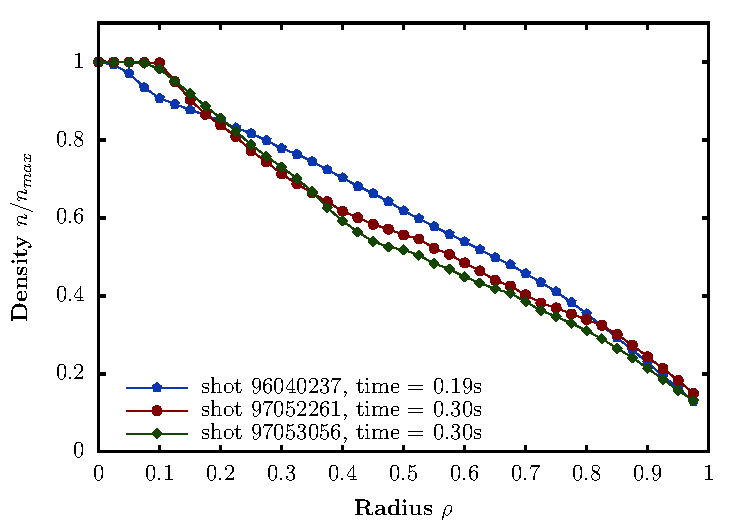
\includegraphics[width=0.5\textwidth]{plots/pr08_rtpn.pdf}
	\caption{Perfiles de densidad electrónica medidos para el Tokamak RTP en diferentes descargas normalizados a la densidad máxima de la descarga. Datos obtenidos de the ITPA International Multi-Tokamak Confinement Profile Database \cite{roach2008}, bajo libre acceso.}
	\label{fig:exp_nprofiles}
\end{figure}

En la Figura \ref{fig:exp_Tprofiles} se tienen los perfiles de temperatura electrónica normalizada medidos para el dispositivo RTP en un tiempo fijo dado.
\begin{figure}[hb!]
	\centering
	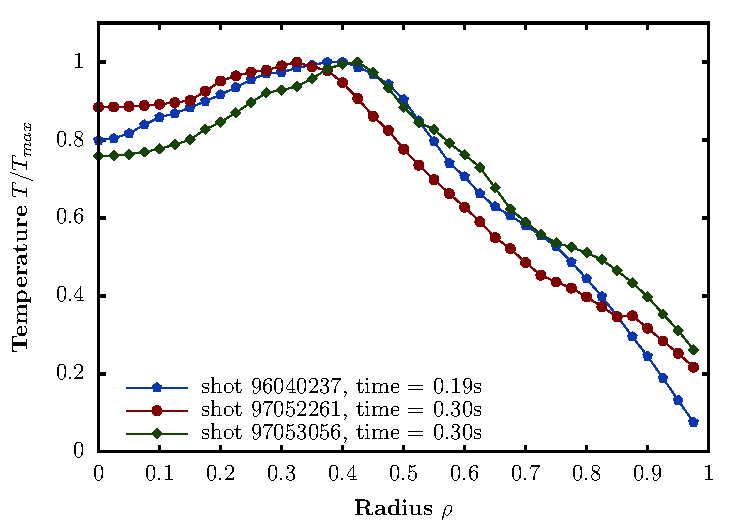
\includegraphics[width=0.5\textwidth]{plots/pr08_rtpT.pdf}
	\caption{Perfiles de temperatura electrónica medidos para el Tokamak RTP en diferentes descargas normalizados a la temperatura máxima de la descarga. Datos obtenidos de the ITPA International Multi-Tokamak Confinement Profile Database \cite{roach2008}, bajo libre acceso.}
	\label{fig:exp_Tprofiles}
\end{figure}

\subsection{Implementación de la red}

Se completo una primera implementación de la PINN usando el paquete \texttt{DeepXDE} \cite{lu2021} de \texttt{Python} con \textit{backend} en \texttt{Pytorch} \cite{pytorch}. Siguiendo los pasos detallados en la metodología. 

\section{Problemáticas}

A lo largo de estas semanas se han podido identificar tres principales problemáticas. La primera con la normalización de las ecuaciones. Se tuvo que normalizar las ecuaciones permitiendo que la temperatura y densidad electrónica tuvieran un mínimo en $T_{min} = 0 \quad eV$ y $n_{min} = 0 \quad cm^{-3}$, lo que teóricamente se puede permitir sabiendo que no va a pasar, pero a nivel de la PINN no es realmente cierto o la forma en que se desearía hacer. No obstante, es la única forma de obtener ecuaciones diferenciales normalizadas y adimensionales. Esto trae algunos problemas con la red neuronal y con posibles puntos de divergencia. Sin embargo, se puede manejar de forma manual para que no llegue a estos extremos. Aún se está tratando de combatir este problema. 

La segunda problemática identificada, es la diferencia en las magnitudes y escalas dentro de las ecuaciones. Esto está trayendo ciertas fluctuaciones numéricas y soluciones no fiables. Se está investigando el trabajo de \cite{chen2026} para obtener ideas de implementación que combatan estos problemas. 

Por último, se están obteniendo perfiles no normalizados, lo que va en contra de las ecuaciones y condiciones de frontera impuestas e implementadas. Se está trabajando activamente en este problema. Se está experimentando con las constantes y con pesos adaptativos dentro de la PINN para obtener algunas respuestas sobre el origen del problema.
 
\section{Cronograma}

\begin{table}[h!]
\caption{Cronograma actualizado de trabajo para el proyecto de investigación.}
\label{tab:cronograma}
\resizebox{0.5\textwidth}{!}{
\begin{tabular}{|l|l|}
\hline
\textbf{Semanas}          & \textbf{Actividad}                                                                                                \\ \hline
25 - 29 mayo & \begin{tabular}[c]{@{}l@{}}Resolver inestabilidades de la PINN. \\Hacer pruebas y obtener perfiles.\end{tabular}       \\ \hline
01 - 15 de junio        & \begin{tabular}[c]{@{}l@{}} Tener listos los datos para comparar \\del objetivo 3 y pulir la PINN\\, obtener perfiles y reajustar \\implementación acordemente\end{tabular}                   \\ \hline
06 - 10 de Julio         & \begin{tabular}[c]{@{}l@{}}Trabajar en la presentación y póster/ \\ Correcciones en el informe final\end{tabular} \\ \hline
\end{tabular}}
\end{table}


%\section{Referencias} %Este comando de sección como tal lo tienen que borrar en su documento (el título de Referencias sale automáticamento con el comando de bibliography

%%%%%%%%%%%%%%%%%%%%%%%%%%%%%%%%%%%%%%%%%%%%%%%%%%%%%%%%%%%%%%%%%%%%%%%%%%%%%%%%%
% Se puede citar un libro o un artículo con el comando: \cite{referencia}.
% Las referencias serán definidas en la bibliografía al final de este archivo .tex, en este plantilla está como sample-paper.bib															
%%%%%%%%%%%%%%%%%%%%%%%%%%%%%%%%%%%%%%%%%%%%%%%%%%%%%%%%%%%%%%%%%%%%%%%%%%%%%%%%%

%%%%%%%%%%%%%%%%%%%%%%%%%%%%%%%%%%%%%%%%%%%%%%%%%%%%%%%%%%%%%%%%%%%%%%%%%%%%%%%%%
% Ahora añadimos el archivo fuente de la bobliografía(sin incluir el .bib)				% 
%%%%%%%%%%%%%%%%%%%%%%%%%%%%%%%%%%%%%%%%%%%%%%%%%%%%%%%%%%%%%%%%%%%%%%%%%%%%%%%%%
%\bibliography{sample-paper}

\bibliography{references}
\bibliographystyle{apsrev4-1}


%%%%%%%%%%%%%%%%%%%%%%%%%%%%%%%%%%%%%%%%%%%%%%%%%%%%%%%%%%%%%%%%%%%%%%%%%%%%%%%%%
%%%%%%%%%%%%%%%%%%%%%%%%%%%%%%%%%%%%%%%%%%%%%%%%%%%%%%%%%%%%%%%%%%%%%%%%%%%%%%%%%
% Otra manera de poner la bibliografía:													%
%																						%
%\bibliographystyle{prsty}																%
%\begin{thebibliography}{99}															%
%\bibitem{melissinos1966}Melissinos, A.C., Experiments in Modern						%
%  Physics - 1st Edition, Academic Press,  [1966]										%
%\bibitem{melissinos2003}Melissinos, A.C., Napolitano, J.,  Experiments in Modern		%
%  Physics - 2nd Edition, Academic Press,  [2003]										%
%\bibitem{bevington2003}Bevington and Robinson, Data Reduction and						%
%  Error Analysis for the Physical Sciences - 3rd Edition, McGraw-Hill,					%
%  [2003]																				%
%\bibitem{pritchard1990}Professor D. Pritchard, Personal Communication					%
%\end{thebibliography}																	%
																						%
%%%%%%%%%%%%%%%%%%%%%%%%%%%%%%%%%%%%%%%%%%%%%%%%%%%%%%%%%%%%%%%%%%%%%%%%%%%%%%%%%
%%%%%%%%%%%%%%%%%%%%%%%%%%%%%%%%%%%%%%%%%%%%%%%%%%%%%%%%%%%%%%%%%%%%%%%%%%%%%%%%%

\clearpage
\appendix


\end{document}
